% start preamble 
\documentclass{article}
\usepackage{graphicx} % Required for inserting images
\usepackage{dsfont}
%\usepackage{parskip}
\usepackage{amsmath}
\graphicspath{ {./pictures/} }


\title{Hausübung Nr. 2}
\author{Sebastian Steitz, Hannes Albert}
\date{April 2023}
% end preamble 
\begin{document}

\maketitle

\section{H2.1}
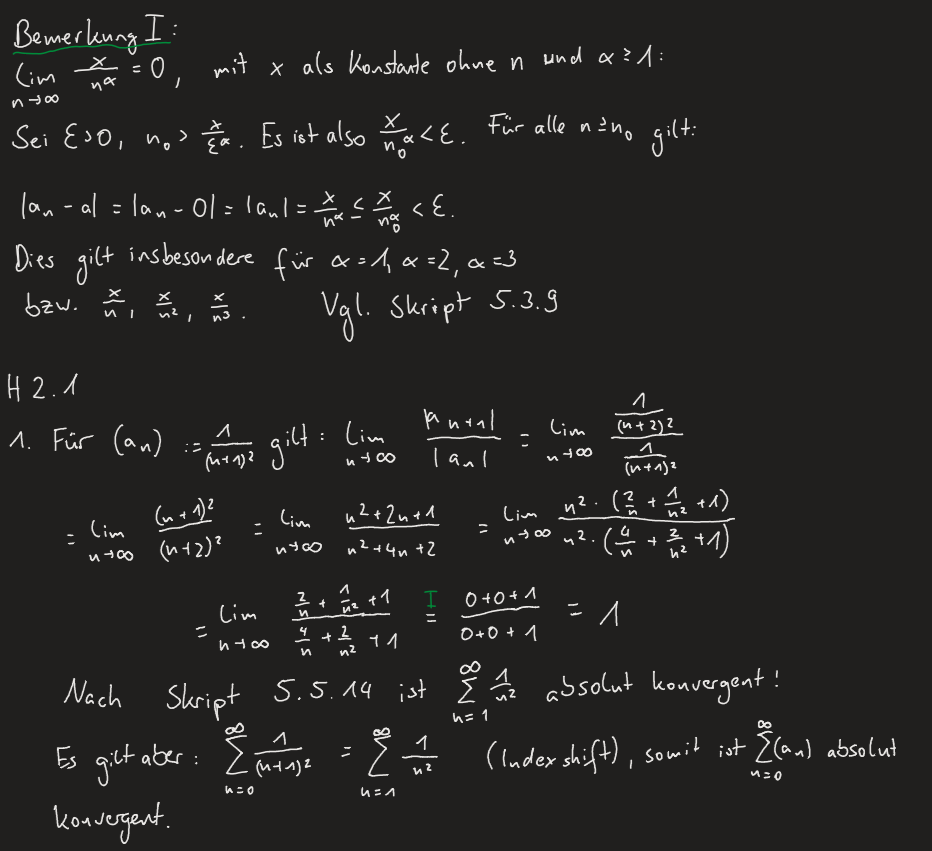
\includegraphics[scale=0.6]{h2_1_1} \\ 

\bigskip
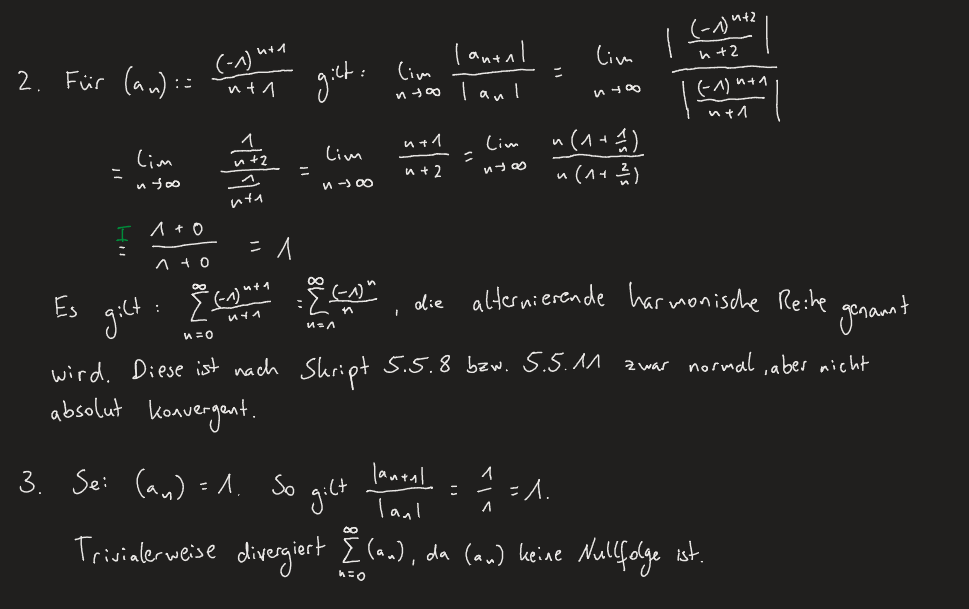
\includegraphics[scale=0.6]{h2_1_2}

\section{H2.2}
\bigskip
1) \\
\setlength\leftskip{1cm}
$O_1 \cup O_2$: \\ 
Nach Definition 5.6.8 müssen wir zeigen, dass es für ein beliebiges \\
a $\in$ $O_1$ $\cup$ $O_2$ ein
r $\in$ $\mathds{R}$ mit $B_r \subseteq O_1 \cup O_2$ \\
Fall 1: a $a \in O_1$ \\ 
Da $O_1$ offen existiert per Definition ein r mit $B_r(a) \subseteq O_1$. Da 
$O_1$ Teilmenge von $O_1 \cup O_2$ gilt: 
\[
    B_r(a) \subseteq O_1 \subseteq O_1 \cup O_2
\]

\noindent Fall 2: $a \in O_2$ \\
Da $O_2$ offen ist existiert per Definition ein r $\in \mathds{R}$ mit $B_r(a) \subseteq O_2$. Da
$O_2$ Teilmenge von $O_1 \cup O_2$ gilt:
\[
    B_r(a) \subseteq O_2 \subseteq O_1 \cup O_2  
\]
Somit ist die Vorraussetzung erfüllt und wir sind fertig.

\noindent $O_1 \cap O_2$: \\ 
Sei a $\in O_1 \cap O_2$. Damit gilt folgendes: 
\[
    a \in O_1 \cup O_2 \leftrightarrow a \in O_1 \wedge a \in O_2
\]
Daraus folgt, dass wir zwei offene Kugeln erzeugen können: Sei $B_d(a) \subseteq O_1$ und 
$B_e(a) \subseteq O_2$. Wir wählen r:= min\{d, e\}. Wir wählen unser r wie folgt:
\begin{align*}
            r:=\left \{\begin{array}{ll} 
                d \indent falls \text{ } d < e \\ 
                e \indent sonst\\ 
     \end{array} \right. 
\end{align*}
Da somit $B_r(a) \subseteq B_d(a)$ bzw. $B_r(a) \subseteq B_e(a)$ gilt $B_r \subseteq O_1 \cap O_2$.
Damit ist $O_1 \cap O_2$ offen.

\bigskip
\noindent 2. \\
$A_1 \cap A_2$ \\ 
Aus der Abschlusseigenschaften von $A_1$ und $A_2$ erhalten wir $\mathds{R^{n}}\backslash A_1$
ist offen und $\mathds{R}^{n} \backslash A_2$ ist offen. Nach 1. gilt somit auch 
$\mathds{R}^{n} \backslash A_1 \cup \mathds{R}^{n} \backslash A_2$ offen. Zusätzlich 
gilt:
\[
    \mathds{R}^{n} \backslash A_1 \cup A_2 \mathds{R}^{n} = \mathds{R}^n \backslash A_1 \cap A_2 
\]
offen. Insbesondere ist $A_1 \cap A_2$ abgeschlossen.

\noindent $A_1 \cup A_2$ \\ 
Aus der Abgeschlossenheit von $A_1$, $A_2$ und a) folgt: \\
$\mathds{R}^{n} \backslash A_1 \cap \mathds{R}^{n} \backslash A_2$ 
offen. Somit gilt \\  
$\mathds{R}^n \backslash A_1 \cap A_2$ offen und $A_1 \cup A_2$ abgeschlossen. 

\bigskip
\noindent 3. \\ 
Induktionsanfang: Sei k $\in \mathds{N}^*$ mit k = 1:
$\overset{1}{\underset{i = 1}{\bigcap}} O_i$ = $O_1$. $O_1$ ist schon per Definiton offen.
\smallskip
Für ein k $\in \mathds{N}^*$ ist  $\overset{k}{\underset{i = 1}{\bigcap}} O_i$ offen.
\smallskip
Induktionsschritt: 
Wir betrachten den Fall k + 1:
\begin{align*}
    \overset{k+1}{\underset{i = 1}{\bigcap}} O_i =                                   
    \overset{k}{\underset{i = 1}{\bigcap}} O_i \cap O_{k + 1} 
\end{align*}
Dass $\overset{k}{\underset{i = 1}{\bigcap}} O_i$ offen ist folgt aus der IV und dass $O_{k + 1}$
offen ist folgt per Definition. Somit sind wir fertig.

\bigskip
\noindent 4. \\ 
Betrachten wir die offene Mengen $O_i$ = (0, $\frac{1}{i}$). So gilt $\overset{k}{\underset{i = 1}{\bigcap}} O_i$ = \{0\}, da die harmonische 
Reihe ($\frac{1}{n}$) gegen 0 geht. \{0\} ist allerdings nicht offen, weshalb es sich hier um ein passendes Gegenbeispiel handelt.

\section{H2.3}
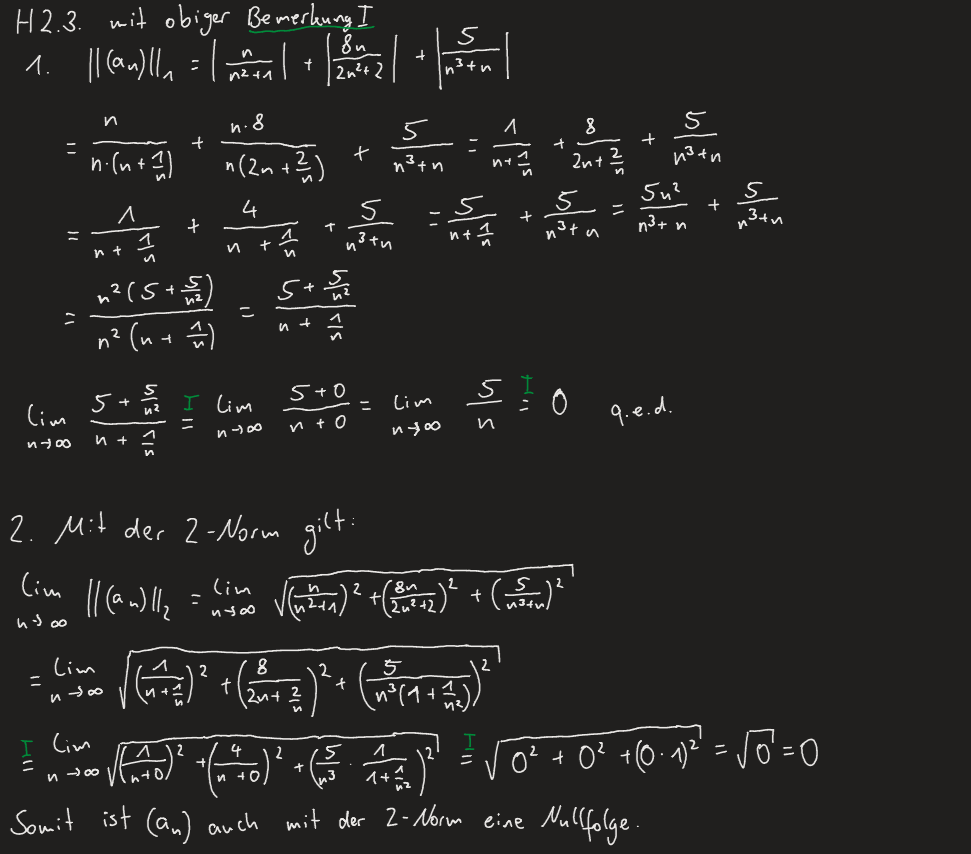
\includegraphics[scale=0.6]{h2_3}


\end{document}
